
\begin{enumerate}
    \item micros\_mars\_task\_alloc

    \acs{ros} has a package, micros\_mars\_task\_alloc, that is used for multi-task allocation. It is based on
    a multi-agent theory using an ALLIANCE model. The ALLIANCE model uses a cooperative robot team where
    each robot is an intelligent agent.
    
    The ALLIANCE model is based on Brooks' subsumption model. A subsumption architecture is a reactive robot architecture that tries to solve 
    the problem of intelligence from a different perspective than traditional AI \cite{ros:micros_mars_task_alloc}. 
    
    \begin{figure}[ht]
        \centering
        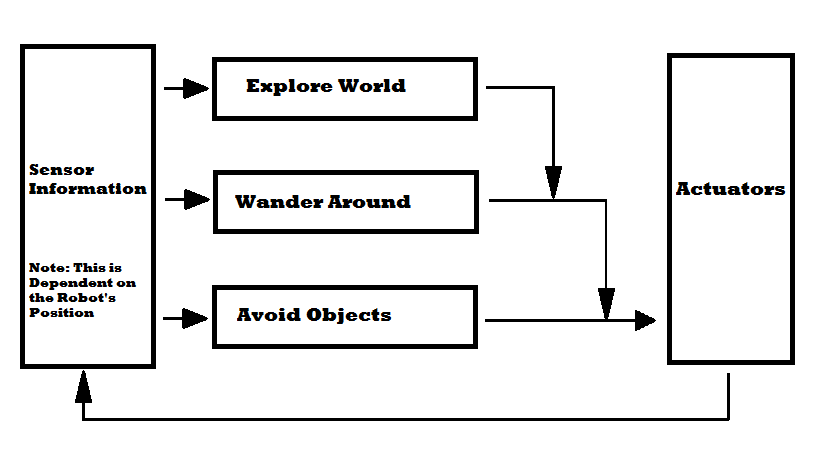
\includegraphics[scale=0.5]{Subsumption_Architecture_Abstract_Diagram.png}
        \caption[Subsumption architecture abstract diagram]{Subsumption architecture abstract diagram\footnotemark.}
    \end{figure}
    
    The ALLIANCE model adds several different behavior sets and behavior layers. These sets and layers are both implemented by following 
    the subsumption model.

    \newpage
    \item FIPA 

    \begin{figure}[ht]
        \centering
        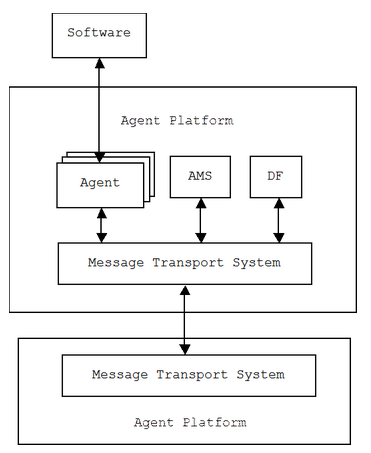
\includegraphics[scale=0.5]{FIPA.png}
        \caption[FIPA]{FIPA diagram\footnotemark.}
    \end{figure}

    \acs{fipa} (Foundation for Intelligent Physical Agents) is an open source agent platform from Nortel Networks. The platform uses an 
    agent communication language that conforms to the \acs{fipa} agent standards. \cite{FIPA-OS}

\end{enumerate}